\documentclass[ignorenonframetext,aspectratio=169]{beamer}
\setbeamertemplate{caption}[numbered]
\setbeamertemplate{caption label separator}{: }
\setbeamercolor{caption name}{fg=normal text.fg}
\beamertemplatenavigationsymbolsempty
\usepackage{lmodern}
\usepackage{amssymb,amsmath}
\usepackage{ifxetex,ifluatex}
\usepackage{fixltx2e} % provides \textsubscript
\ifnum 0\ifxetex 1\fi\ifluatex 1\fi=0 % if pdftex
  \usepackage[T1]{fontenc}
  \usepackage[utf8]{inputenc}
\else % if luatex or xelatex
  \ifxetex
    \usepackage{mathspec}
  \else
    \usepackage{fontspec}
  \fi
  \defaultfontfeatures{Ligatures=TeX,Scale=MatchLowercase}
\fi
% use upquote if available, for straight quotes in verbatim environments
\IfFileExists{upquote.sty}{\usepackage{upquote}}{}
% use microtype if available
\IfFileExists{microtype.sty}{%
\usepackage{microtype}
\UseMicrotypeSet[protrusion]{basicmath} % disable protrusion for tt fonts
}{}
\newif\ifbibliography
\hypersetup{
            pdftitle={Unit 3: Distributions},
            pdfauthor={Statistics 102 Teaching Team},
            pdfborder={0 0 0},
            breaklinks=true}
\urlstyle{same}  % don't use monospace font for urls
\usepackage{color}
\usepackage{fancyvrb}
\newcommand{\VerbBar}{|}
\newcommand{\VERB}{\Verb[commandchars=\\\{\}]}
\DefineVerbatimEnvironment{Highlighting}{Verbatim}{commandchars=\\\{\}}
% Add ',fontsize=\small' for more characters per line
\usepackage{framed}
\definecolor{shadecolor}{RGB}{248,248,248}
\newenvironment{Shaded}{\begin{snugshade}}{\end{snugshade}}
\newcommand{\KeywordTok}[1]{\textcolor[rgb]{0.13,0.29,0.53}{\textbf{#1}}}
\newcommand{\DataTypeTok}[1]{\textcolor[rgb]{0.13,0.29,0.53}{#1}}
\newcommand{\DecValTok}[1]{\textcolor[rgb]{0.00,0.00,0.81}{#1}}
\newcommand{\BaseNTok}[1]{\textcolor[rgb]{0.00,0.00,0.81}{#1}}
\newcommand{\FloatTok}[1]{\textcolor[rgb]{0.00,0.00,0.81}{#1}}
\newcommand{\ConstantTok}[1]{\textcolor[rgb]{0.00,0.00,0.00}{#1}}
\newcommand{\CharTok}[1]{\textcolor[rgb]{0.31,0.60,0.02}{#1}}
\newcommand{\SpecialCharTok}[1]{\textcolor[rgb]{0.00,0.00,0.00}{#1}}
\newcommand{\StringTok}[1]{\textcolor[rgb]{0.31,0.60,0.02}{#1}}
\newcommand{\VerbatimStringTok}[1]{\textcolor[rgb]{0.31,0.60,0.02}{#1}}
\newcommand{\SpecialStringTok}[1]{\textcolor[rgb]{0.31,0.60,0.02}{#1}}
\newcommand{\ImportTok}[1]{#1}
\newcommand{\CommentTok}[1]{\textcolor[rgb]{0.56,0.35,0.01}{\textit{#1}}}
\newcommand{\DocumentationTok}[1]{\textcolor[rgb]{0.56,0.35,0.01}{\textbf{\textit{#1}}}}
\newcommand{\AnnotationTok}[1]{\textcolor[rgb]{0.56,0.35,0.01}{\textbf{\textit{#1}}}}
\newcommand{\CommentVarTok}[1]{\textcolor[rgb]{0.56,0.35,0.01}{\textbf{\textit{#1}}}}
\newcommand{\OtherTok}[1]{\textcolor[rgb]{0.56,0.35,0.01}{#1}}
\newcommand{\FunctionTok}[1]{\textcolor[rgb]{0.00,0.00,0.00}{#1}}
\newcommand{\VariableTok}[1]{\textcolor[rgb]{0.00,0.00,0.00}{#1}}
\newcommand{\ControlFlowTok}[1]{\textcolor[rgb]{0.13,0.29,0.53}{\textbf{#1}}}
\newcommand{\OperatorTok}[1]{\textcolor[rgb]{0.81,0.36,0.00}{\textbf{#1}}}
\newcommand{\BuiltInTok}[1]{#1}
\newcommand{\ExtensionTok}[1]{#1}
\newcommand{\PreprocessorTok}[1]{\textcolor[rgb]{0.56,0.35,0.01}{\textit{#1}}}
\newcommand{\AttributeTok}[1]{\textcolor[rgb]{0.77,0.63,0.00}{#1}}
\newcommand{\RegionMarkerTok}[1]{#1}
\newcommand{\InformationTok}[1]{\textcolor[rgb]{0.56,0.35,0.01}{\textbf{\textit{#1}}}}
\newcommand{\WarningTok}[1]{\textcolor[rgb]{0.56,0.35,0.01}{\textbf{\textit{#1}}}}
\newcommand{\AlertTok}[1]{\textcolor[rgb]{0.94,0.16,0.16}{#1}}
\newcommand{\ErrorTok}[1]{\textcolor[rgb]{0.64,0.00,0.00}{\textbf{#1}}}
\newcommand{\NormalTok}[1]{#1}
\usepackage{graphicx,grffile}
\makeatletter
\def\maxwidth{\ifdim\Gin@nat@width>\linewidth\linewidth\else\Gin@nat@width\fi}
\def\maxheight{\ifdim\Gin@nat@height>\textheight0.8\textheight\else\Gin@nat@height\fi}
\makeatother
% Scale images if necessary, so that they will not overflow the page
% margins by default, and it is still possible to overwrite the defaults
% using explicit options in \includegraphics[width, height, ...]{}
\setkeys{Gin}{width=\maxwidth,height=\maxheight,keepaspectratio}

% Prevent slide breaks in the middle of a paragraph:
\widowpenalties 1 10000
\raggedbottom

\AtBeginPart{
  \let\insertpartnumber\relax
  \let\partname\relax
  \frame{\partpage}
}
\AtBeginSection{
  \ifbibliography
  \else
    \let\insertsectionnumber\relax
    \let\sectionname\relax
    \frame{\sectionpage}
  \fi
}
\AtBeginSubsection{
  \let\insertsubsectionnumber\relax
  \let\subsectionname\relax
  \frame{\subsectionpage}
}

\setlength{\parindent}{0pt}
\setlength{\parskip}{6pt plus 2pt minus 1pt}
\setlength{\emergencystretch}{3em}  % prevent overfull lines
\providecommand{\tightlist}{%
  \setlength{\itemsep}{0pt}\setlength{\parskip}{0pt}}
\setcounter{secnumdepth}{0}
\usepackage{amsmath,verbatim}

\usepackage{multirow}
\usepackage{fancyvrb}
\usepackage{manfnt}
\usepackage[normalem]{ulem}

\usepackage{hyperref}
\hypersetup{
	colorlinks,
	linkcolor={blue!50!black},
	urlcolor={blue!80!black}
}

%\usepackage[colorlinks=true]{hyperref}

\mode<presentation>{\usetheme{Malmoe}}

%\synctex=1

\setbeamertemplate{headline}{}


\setbeamerfont{footline}{size=\scriptsize}
\setbeamerfont{frametitle}{shape=\scshape}
\setbeamertemplate{itemize items}[circle]
\setbeamercovered{transparent}

\setbeamertemplate{navigation symbols}{}
\setbeamertemplate{footline}[frame number]{} 


\definecolor{forest}{rgb}{0, .5, 0}
\definecolor{brick}{rgb}{.5, 0, 0}
\definecolor{darkgreen}{rgb}{0, .5, 0}
\definecolor{darkred}{rgb}{.7, .15, .15}
\definecolor{darkblue}{rgb}{0, 0, .5}
\definecolor{Green}{rgb}{0.2,1,0.2}


\newcommand{\R}{\textsf{R}}
\newcommand{\RStudio}{\textsl{R Studio}}


\usepackage[english]{babel}
%\usepackage{palatino}
\usepackage[T1]{fontenc}


% make all tt fonts bold to look more like Verbatim
\usepackage{lmodern}
\renewcommand\ttfamily{\usefont{T1}{lmtt}{m}{n}}

% Comment these out if you don't want a slide with just the
% part/section/subsection/subsubsection title:
\AtBeginPart{
  \let\insertpartnumber\relax
  \let\partname\relax
  \frame{\partpage}
}
\AtBeginSection{
  \let\insertsectionnumber\relax
  \let\sectionname\relax
  \frame{\sectionpage}
}
\AtBeginSubsection{
  \let\insertsubsectionnumber\relax
  \let\subsectionname\relax
  \frame{\subsectionpage}
}

\newenvironment{twocol}[4]{
\begin{columns}[c]
\column{#1\textwidth}
#3
\column{#2\textwidth}
#4
\end{columns}
}

\def\begincols{\begin{columns}}
\def\begincol{\begin{column}}
\def\endcol{\end{column}}
\def\endcols{\end{columns}}

\title{Unit 3: Distributions}
\author{Statistics 102 Teaching Team}
\date{February 17, 2020}

\begin{document}
\frame{\titlepage}

\begin{frame}
\tableofcontents[hideallsubsections]
\end{frame}

\section{Random Variables}\label{random-variables}

\begin{frame}{Main ideas this section}

\begin{itemize}
\item
  Definition of random variables
\item
  Distributions of random variables
\item
  Mean, variance, and standard deviation for random variables
\end{itemize}

\end{frame}

\begin{frame}{Definition of a Random Variable}

A \emph{random variable} is a function that maps each event in a sample
space to a number.

\begin{itemize}
\tightlist
\item
  A \emph{discrete random variable} takes on a finite number of values.
\end{itemize}

Suppose \(X\) is the number of heads in 3 tosses of a fair coin.

\begin{itemize}
\tightlist
\item
  \(X\) can take on the values 0, 1, 2, 3.
\end{itemize}

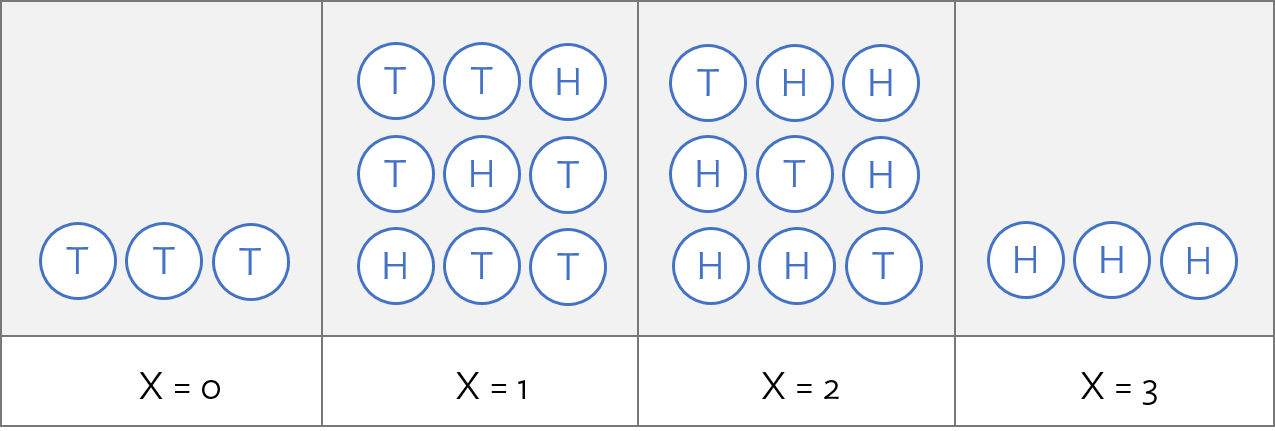
\includegraphics{figures/coinToss.png}

\end{frame}

\begin{frame}{Distribution of a Discrete Random Variable}

The distribution of a discrete random variable is the collection of its
values and the probabilities associated with those values.

The probability distribution for \(X\) is as follows:

\centering

\begin{tabular}{l | rrrr }
        $x_i$ & 0 & 1 & 2 & 3 \\
        \hline
        $P(X = x_i)$ & 1/8 & 3/8 & 3/8 & 1/8 \\
    \end{tabular}

\[\sum_{x=0}^3 P(X = x_i) = 1 \]

\end{frame}

\begin{frame}{Bar graph showing a distribution}

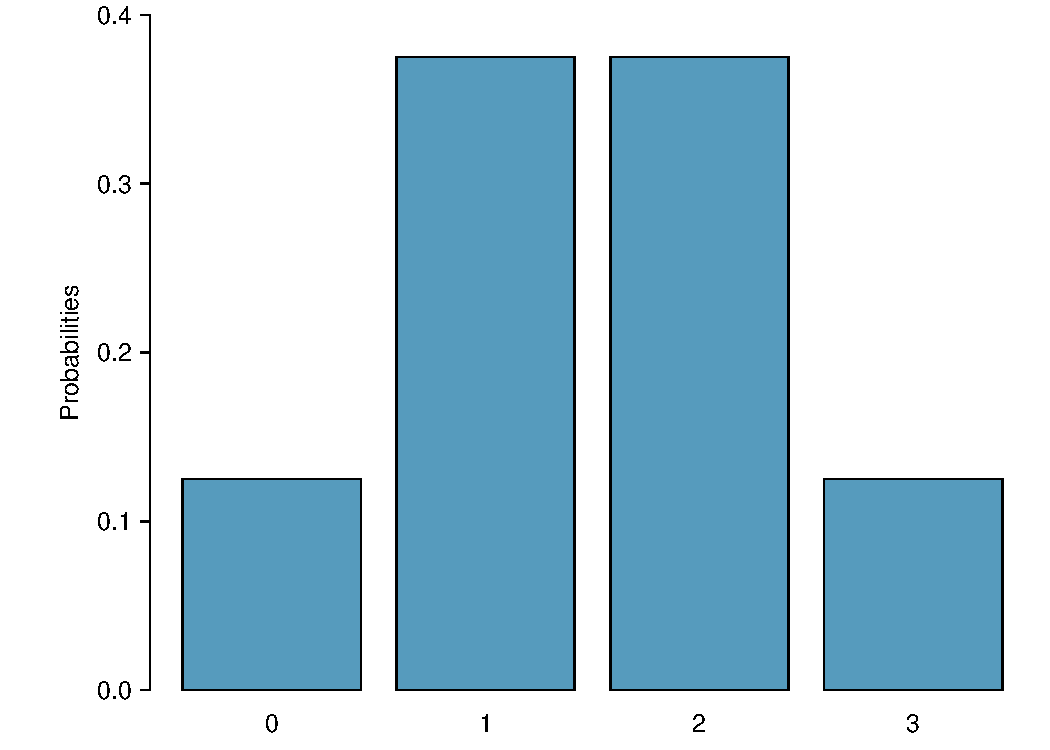
\includegraphics{figures/barPlotCoinTossing.pdf}

\end{frame}

\begin{frame}{Using a simulation to construct a probability
distribution}

Distributions of random variables that arise in science can be more
complex.

In lab, we will run a simulation to view the distribution of good
responses in a clinical trial with 8 participants, under the assumption
that the probability of a good response is 0.15.

\end{frame}

\begin{frame}{Expectation of a Random Variable}

If \(X\) has outcomes \(x_1\), \ldots{}, \(x_k\) with probabilities
\(P(X=x_1)\), \ldots{}, \(P(X=x_k)\), the expected value of \(X\) is the
sum of each outcome multiplied by its corresponding probability:
\[E(X)  = x_1 P(X=x_1) + \cdots + x_k P(X=x_k) = \sum_{i=1}^{k}x_iP(X=x_i)\]
The Greek letter \(\mu\) may be used in place of the notation \(E(X)\)
and is sometimes written \(\mu_X\).

\end{frame}

\begin{frame}{Expectation\ldots{}}

In the coin tossing example,

\begin{align*}
E(X) &= 0P(X=0) + 1P(X=1) + 2P(X=2) + 3P(X = 3)  \\
    &= (0)(1/8) + (1)(3/8) + (2)(3/8) + (3)(1/8)  \\
    &= 12/8  \\
    &= 1.5 
\end{align*}

\end{frame}

\begin{frame}{Variance and SD of a Random Variable}

If \(X\) takes on outcomes \(x_1\), \ldots{}, \(x_k\) with probabilities
\(P(X=x_1)\), \ldots{}, \(P(X=x_k)\) and expected value \(\mu=E(X)\),
then the variance of \(X\), denoted by \(\text{Var}(X)\) or
\(\sigma^2\), is

\begin{align*}
\text{Var}(X) &= (x_1-\mu)^2 P(X=x_1) + \cdots+ (x_k-\mu)^2 P(X=x_k) \\
    &= \sum_{j=1}^{k} (x_j - \mu)^2 P(X=x_j)
\end{align*}

The standard deviation of \(X\), written as \(\text{SD}(X)\) or
\(\sigma\), is the square root of the variance. It is sometimes written
\(\sigma_X\).

\end{frame}

\begin{frame}{Variance and SD\ldots{}}

In the coin tossing example,

\begin{align}
    \sigma_X^2 &= (x_1-\mu_X)^2P(X=x_1) + \cdots+ (x_4-\mu)^2 P(X=x_4) \notag \\
        &= (0- 1.5)^2(1/8) + (1 - 1.5)^2 (3/8) + (2 -1.5)^2 (3/8) + (3-1.5)^2 (1/8) \notag  \\
        &= 3/4 \notag
    \end{align}

The standard deviation is \(\sqrt{3/4} = \sqrt{3}/2 = 0.866\).

\end{frame}

\section{The Binomial distribution}\label{the-binomial-distribution}

\begin{frame}{Binomial Random Variables}

One specific type of discrete random variable is a binomial random
variable.

\(X\) is a binomial random variable if it represents the number of
successes in \(n\) independent replications of an experiment where

\begin{itemize}
\tightlist
\item
  Each replicate has two possible outcomes: either success or failure
\item
  The probability of success \(p\) in each replicate is constant
\end{itemize}

A binomial random variable takes on values \(0, 1, 2, \dots, n\).

The number of heads in 3 tosses of a fair coin is a binomial random
variable with parameters \(n = 3\) and \(p = 0.5\).

\end{frame}

\begin{frame}{The Binomial Coefficient}

The binomial coefficient \(\binom{n}{x}\) is the number of ways to
choose \(x\) items from a set of size \(n\), where the order of the
choice is ignored.

Mathematically,

\[\binom{n} {x} = \frac{n!}{x!(n-x)!}\]

\begin{itemize}
\item
  \(n = 1, 2, \ldots\)
\item
  \(x = 0, 1, 2, \ldots, n\)
\item
  For any integer \(m\), \(m! = (m)(m-1)(m-2)\cdots(1)\)
\end{itemize}

\end{frame}

\begin{frame}{Formula for the binomial distribution}

Let \(x\) = number of successes in \(n\) trials

\begin{footnotesize}
\[P(x \,\,\text{successes}) = \binom{\text{\# of trials}} 
   {\text{\# of successes}} 
   p^{\text{\# of successes}}(1-p)^{\text{\# of trials - \# of successes}}\]
\end{footnotesize}

\[P(X = x)=\binom{n}{x} p^x (1-p)^{n-x},\:  x= 0, 1, 2, \dots, n\]

\emph{Parameters of the distribution}:

\begin{itemize}
\item
  \(n\) = number of trials
\item
  \(p\) = probability of success
\end{itemize}

Shorthand notation: \(X\sim \text{Bin}(n,p)\)

\end{frame}

\begin{frame}{Mean and SD for a binomial random variable}

For a binomial distribution with parameters \(n\) and \(p\), it can be
shown that:

\begin{itemize}
\item
  Mean = \(np\) \medskip 
\item
  Standard Deviation = \(\sqrt{np(1-p)}\) \medskip 
\end{itemize}

The derivation is not shown here nor in the text; it will not be asked
for on a problem set or exam.

\end{frame}

\begin{frame}{Calculating binomial probabilities in \textsf{R}}

The function \texttt{dbinom()} is used to calculate \(P(X = k)\).

\begin{itemize}
\tightlist
\item
  \texttt{dbinom(k, n, p)}: \(P(X = k)\)
\end{itemize}

The function \texttt{pbinom()} is used to calculate \(P(X \leq k)\) or
\(P(X > k)\).

\begin{itemize}
\item
  \texttt{pbinom(k, n, p)}: \(P(X \leq k)\)
\item
  \texttt{pbinom(k, n, p, lower.tail = FALSE)}: \(P(X > k)\)
\end{itemize}

\end{frame}

\section{The Normal distribution}\label{the-normal-distribution}

\begin{frame}{Continuous random variables}

A discrete random variable takes on a finite number of values.

\begin{itemize}
\item
  Number of heads in a set of coin tosses
\item
  Number of people who have had chicken pox in a random sample
\end{itemize}

A continuous random variable can take on any real value in an interval.

\begin{itemize}
\item
  Height in a population
\item
  Blood pressure in a population
\end{itemize}

A general distinction to keep in mind: discrete random variables are
\emph{counted}, but continuous random variables are \emph{measured}.

\end{frame}

\begin{frame}{Probabilities for continuous distributions}

Two important features of continuous distributions:

\begin{itemize}
\item
  The total area under the density curve is 1.
\item
  The probability that a variable has a value within a specified
  interval is the area under the curve over that interval.
\end{itemize}

\begin{center}
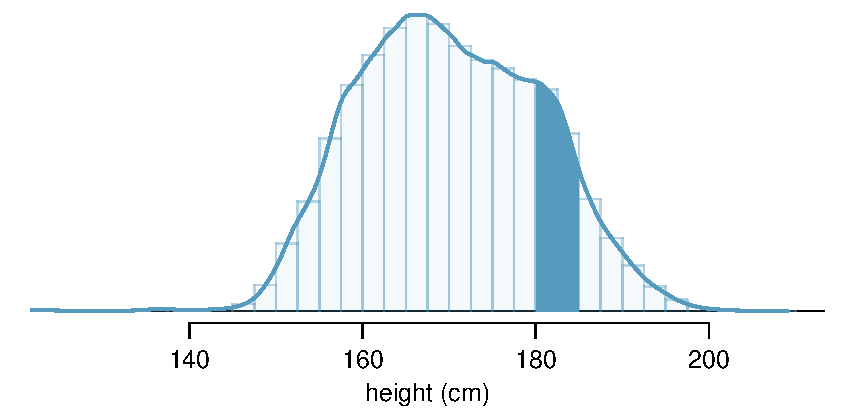
\includegraphics[width=4in]{figures/fdicHeightContDistFilled.pdf}
\end{center}

\end{frame}

\begin{frame}{Probabilities for continuous distributions\ldots{}}

When working with continuous random variables, probability is found for
intervals of values rather than individual values.

\begin{itemize}
\item
  The probability that a continuous r.v. \(X\) takes on any single
  individual value is 0. That is, \(P(X = x) = 0\).
\item
  Thus, \(P(a < X < b)\) is equivalent to \(P(a \leq X \leq b)\).
\end{itemize}

\end{frame}

\begin{frame}{The normal distribution}

According to the Empirical Rule, for any normal distribution,

\begin{itemize}
\item
  approximately 68\% of the data are within 1 SD of the mean \medskip 
\item
  approximately 95\% of the data are within 2 SDs of the mean \medskip
\item
  approximately 99.7\% of the data are within 3 SDs of the mean
\end{itemize}

\centering
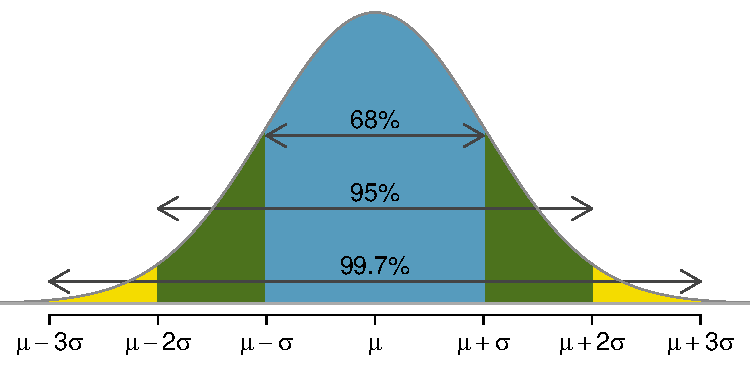
\includegraphics[width=0.75000\textwidth]{./figures/6895997.pdf}

\end{frame}

\begin{frame}{A Normal Example}

The distribution of test scores on the SAT and the ACT are both nearly
normal.

Suppose that one student scores an 1800 on the SAT (Student A) and
another student scores a 24 on the ACT (Student B). Which student
performed better?

\begin{figure}[]
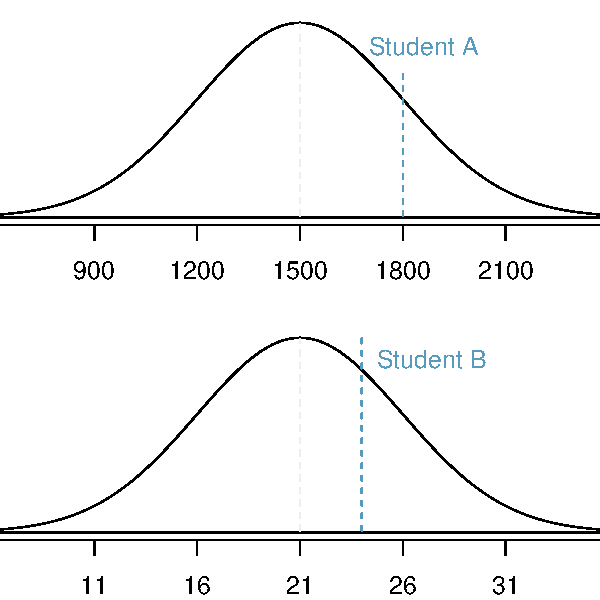
\includegraphics[width=0.4\textwidth]
{./figures/satActNormals.pdf}
\end{figure}

\end{frame}

\begin{frame}{Standard Normal Distribution}

A \emph{standard normal} distribution is defined as a normal
distribution with mean 0 and variance 1. It is often denoted as
\(Z \sim N(0, 1)\).

Any normal random variable \(X\) can be transformed into a standard
normal random variable \(Z\).

\[Z = \dfrac{X - \mu}{\sigma} \qquad X = \mu + Z\sigma \]

\end{frame}

\begin{frame}{A Normal Example\ldots{}}

\begin{itemize}
\item
  SAT scores are \(N(1500, 300)\). ACT scores are \(N(21,5)\).
\item
  \(x_A\) represents the score of Student A; \(x_B\) represents the
  score of Student B.
\end{itemize}

\[Z_{A} = \frac{x_{A} - \mu_{SAT}}{\sigma_{SAT}} = \frac{1800-1500}{300} = 1 \]

\[Z_{B} = \frac{x_{B} - \mu_{ACT}}{\sigma_{ACT}} = \frac{24 - 21}{5} = 0.6\]

\end{frame}

\begin{frame}[fragile]{Calculating Normal Probabilities (I)}

What is the percentile rank for a student who scores an 1800 on the SAT
for a year in which the scores are \(N(1500, 300)\)?

\footnotesize

\begin{enumerate}
\def\labelenumi{\arabic{enumi}.}
\item
  Calculate a \(Z\)-score. If \(X\) is a normal random variable with
  mean \(\mu\) and standard deviation \(\sigma\),
  \[Z = \frac{X - \mu}{\sigma},  \] is a standard normal random variable
  (\(\mu = 0\), \(\sigma =1\)).
\item
  Calculate the normal probability.

  \begin{itemize}
  \tightlist
  \item
    \texttt{pnorm(z)} calculates the area (i.e., probability) to the
    left of \(z\)
  \end{itemize}

\begin{Shaded}
\begin{Highlighting}[]
\KeywordTok{pnorm}\NormalTok{(}\DecValTok{1}\NormalTok{)}
\end{Highlighting}
\end{Shaded}

\begin{verbatim}
## [1] 0.8413447
\end{verbatim}
\item
  Alternatively, let \textsf{R} do the work \ldots{}

\begin{Shaded}
\begin{Highlighting}[]
\KeywordTok{pnorm}\NormalTok{(}\DecValTok{1800}\NormalTok{, }\DecValTok{1500}\NormalTok{, }\DecValTok{300}\NormalTok{)}
\end{Highlighting}
\end{Shaded}

\begin{verbatim}
## [1] 0.8413447
\end{verbatim}
\end{enumerate}

\end{frame}

\begin{frame}[fragile]{Calculating Normal Probabilities (II)}

What score on the SAT would put a student in the 99\(^{th}\) percentile?

\footnotesize

\begin{enumerate}
\def\labelenumi{\arabic{enumi}.}
\item
  Identify the \(Z\)-value. \texttt{qnorm(p)} calculates the value \(z\)
  such that for a standard normal variable \(Z\), \(p = P(Z \leq z)\).

\begin{Shaded}
\begin{Highlighting}[]
\KeywordTok{qnorm}\NormalTok{(}\FloatTok{0.99}\NormalTok{)}
\end{Highlighting}
\end{Shaded}

\begin{verbatim}
## [1] 2.326348
\end{verbatim}
\item
  Calculate the score, \(X\). If \(Z\) is distributed standard Normal,
  then \[X = \sigma Z + \mu,\] is Normal with mean \(\mu\) and standard
  deviation \(\sigma\).
\end{enumerate}

\[X = \sigma Z + \mu = 300(2.33) + 1500 = 2199\]

\begin{enumerate}
\def\labelenumi{\arabic{enumi}.}
\setcounter{enumi}{2}
\item
  Alternatively, let \textsf{R} do the work \ldots{}

\begin{Shaded}
\begin{Highlighting}[]
\KeywordTok{qnorm}\NormalTok{(}\FloatTok{0.99}\NormalTok{, }\DecValTok{1500}\NormalTok{, }\DecValTok{300}\NormalTok{)}
\end{Highlighting}
\end{Shaded}

\begin{verbatim}
## [1] 2197.904
\end{verbatim}
\end{enumerate}

\end{frame}

\section{The Poisson distribution}\label{the-poisson-distribution}

\begin{frame}{Introduction to the Poisson distribution}

The Poisson distribution is used to calculate probabilities for rare
events that accumulate over time.

It used most often in settings where events happen at a rate \(\lambda\)
per unit of population and per unit time, such as the annual incidence
of a disease in a population.

\begin{itemize}
\item
  Typical example: for children ages 0 - 14, the incidence rate of acute
  lymphocytic leukemia (ALL) was approximately 30 diagnosed cases per
  million children per year in 2010.
\item
  Always take care to note and understand the units.
\end{itemize}

\end{frame}

\begin{frame}{Example: Outbreaks of childhood leukemia}

Fortunately, childhood cancers are rare.

For children ages 0 - 14, the incidence rate of acute lymphocytic
leukemia (ALL) was approximately 30 diagnosed cases per million children
per year in the decade from 2000 - 2010. Approximately 20\% of the US
population are in this age range.

\begin{itemize}
\tightlist
\item
  What is the incidence rate over a 5 year period?
\item
  In a small city of 75,000 people, what is the probability of observing
  exactly 8 cases of ALL over a 5 year period?
\item
  In the small city, what is the probability of observing 8 or more
  cases over a 5 year period?
\end{itemize}

\end{frame}

\begin{frame}{Poisson Distribution}

Suppose events occur over time in such a way that

\begin{enumerate}
\def\labelenumi{\arabic{enumi}.}
\item
  The probability an event occurs in an interval is proportional to the
  length of the interval.
\item
  Events occur independently at a rate \(\lambda\) per unit of time.
\end{enumerate}

Then the probability of exactly \(x\) events in one unit of time is \[
P(X = x) = \frac{e^{-\lambda}\lambda^{x}}{x!}, \,\, x = 0, 1, 2,
\ldots
\]

The probability of exactly \(x\) events \(t\) units of time is \[
P(X = x) = \frac{e^{-\lambda t}(\lambda t)^{x}}{x!}, \,\, x = 0, 1,
2, \ldots
\]

Derivation given in more theoretical courses, such as Stat 110.

\end{frame}

\begin{frame}{Poisson distribution with \(\lambda = 2.25\)}

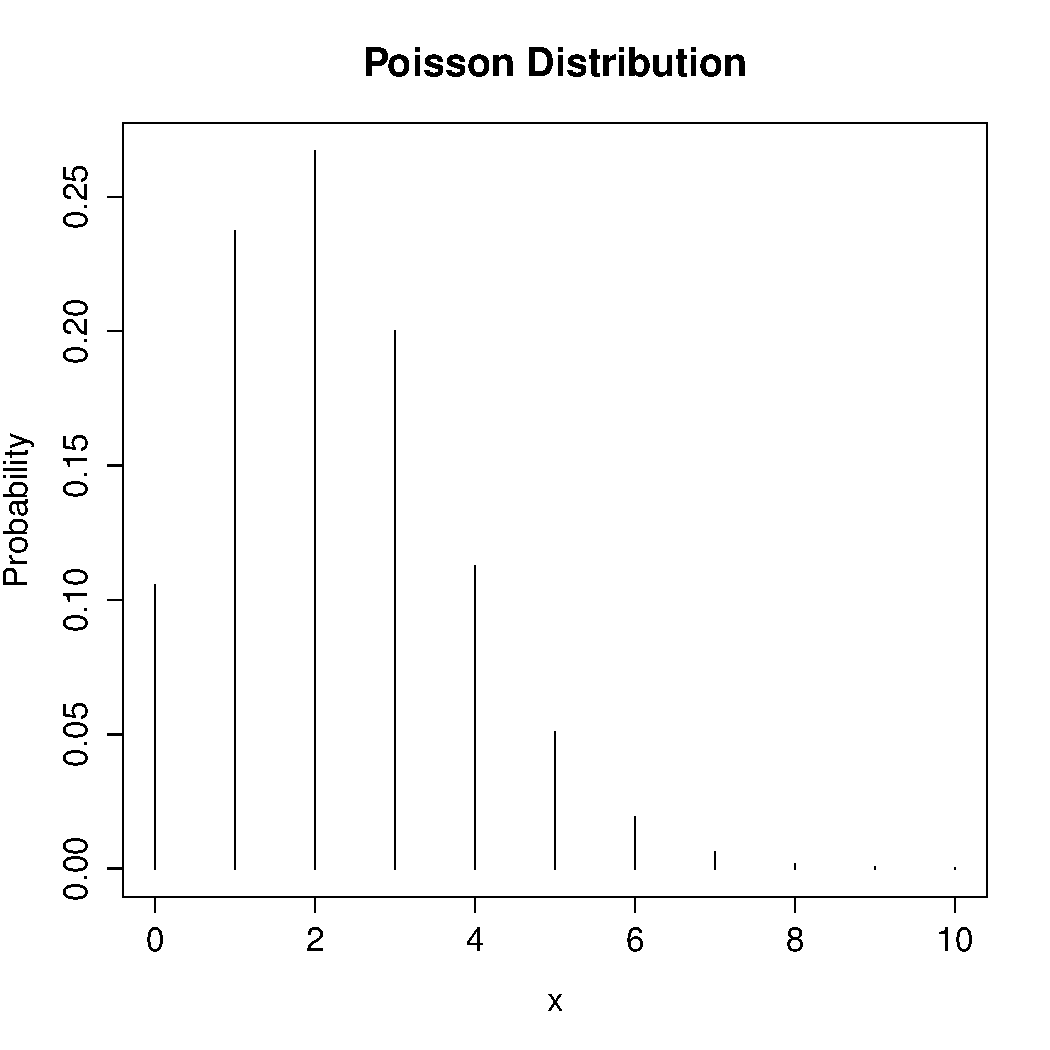
\includegraphics{./figures/pois_2_25.pdf}

\end{frame}

\begin{frame}{Poisson mean and standard deviation}

For the Poisson distribution modeling the number of events in one unit
of time:

\begin{itemize}
\item
  The mean is \(\lambda\).
\item
  The standard deviation is \(\sqrt{\lambda}\).
\end{itemize}

In \(t\) units of time, the mean and standard deviation are,
respectively, \(\lambda t\) and \(\sqrt{\lambda t}\).

\end{frame}

\begin{frame}{Childhood leukemia cases (\emph{OI Biostat}, Example
3.37)}

The incidence rate of ALL in a year is 30 per 1,000,000 children:

\begin{itemize}
\tightlist
\item
  \(\dfrac{30}{1,000,000}= 0.00003 = 3\times 10^{-5}\).
\end{itemize}

The incidence rate over a 5-year period is (5)(30) per 1,000,000
children:

\begin{itemize}
\tightlist
\item
  \(\dfrac{150}{1,000,000} = 0.00015 = 1.5 \times 10^{-4}\).
\end{itemize}

\end{frame}

\begin{frame}{What about a city of size 75,000?}

In a city of 75,000 people, approximately \((75,000)(0.20) = 15,000\)
children will be age 0 - 14 (from slide 31).

The five-year rate of new cases for the city would be:

\[(1.5 \times 10^{-4})(15,000) = 2.25\]

\end{frame}

\begin{frame}[fragile]{What is the probability of 8 cases over 5 years?}

\[P(X=8) = \frac{e^{-\lambda}\lambda^{x}}{x!} =  \frac{e^{(-2.25)}(2.25)^{8}}{8!}\]

Easiest to calculate this in \textsf{R} \ldots{}

Suppose \(X\) has a Poisson distribution with parameter \(\lambda\).

\begin{itemize}
\tightlist
\item
  \texttt{dpois(k, lambda)}: \(P(X = k)\)
\end{itemize}

\begin{Shaded}
\begin{Highlighting}[]
\KeywordTok{dpois}\NormalTok{(}\DecValTok{8}\NormalTok{, }\DataTypeTok{lambda =} \FloatTok{2.25}\NormalTok{)}
\end{Highlighting}
\end{Shaded}

\begin{verbatim}
## [1] 0.001717027
\end{verbatim}

\end{frame}

\begin{frame}[fragile]{What is the probability of 8 or more cases?}

Would 8 or more cases be a rare event?

\begin{itemize}
\tightlist
\item
  Calculate \(P(X \geq 8) = 1 - P(X \leq 7)\).
\end{itemize}

Suppose \(X\) has a Poisson distribution with parameter \(\lambda\).

\footnotesize

\begin{itemize}
\tightlist
\item
  \texttt{ppois(k, lambda)}: \(P(X \leq k)\)
\end{itemize}

\begin{Shaded}
\begin{Highlighting}[]
\DecValTok{1} \OperatorTok{-}\StringTok{ }\KeywordTok{ppois}\NormalTok{(}\DecValTok{7}\NormalTok{, }\DataTypeTok{lambda =} \FloatTok{2.25}\NormalTok{)}
\end{Highlighting}
\end{Shaded}

\begin{verbatim}
## [1] 0.002267088
\end{verbatim}

\begin{itemize}
\tightlist
\item
  \texttt{ppois(k, lambda, lower.tail = FALSE)}: \(P(X > k)\)
\end{itemize}

\begin{Shaded}
\begin{Highlighting}[]
\KeywordTok{ppois}\NormalTok{(}\DecValTok{7}\NormalTok{, }\DataTypeTok{lambda =} \FloatTok{2.25}\NormalTok{, }\DataTypeTok{lower.tail =} \OtherTok{FALSE}\NormalTok{)}
\end{Highlighting}
\end{Shaded}

\begin{verbatim}
## [1] 0.002267088
\end{verbatim}

\end{frame}

\begin{frame}{Distributions Summary Table}

\begin{tabular}{l|ccc} 
  & \textbf{Binomial} & \textbf{Normal} & \textbf{Poisson} \\ \hline
  \textbf{Parameters} & $n$, $p$  & $\mu$,  $\sigma$ & $\lambda$ \\ 
  \textbf{Possible values} & $0,1,\ldots,n$ & (-$\infty$, $\infty$) & $0,1,\ldots,\infty$ \\
  \textbf{Mean} &  $np$  & $\mu$ & $\lambda$ \\ 
  \textbf{Standard Deviation} & $\sqrt{np(1-p)}$ & $\sigma$ & $\sqrt{\lambda}$ \\ 
\end{tabular}

\end{frame}

\end{document}
